%%%--------------------------------%%%
%%% Conception
%%%--------------------------------%%%
\newpage

\section{Gamification}
\label{sec:domainC}

\spacing{1.5}

The gamification conception is based on the gamification design process described in chapter \ref{sec:theoryBd}. Therefore the following chapters deal with the player (chapter \ref{sec:domainCa}), the mission (chapter \ref{sec:domainCb}), the mechanics (chapter \ref{sec:domainCc}) and the evaluation (chapter \ref{sec:domainCd}).

\subsection{Player Personas}
\label{sec:domainCa}

By the initial survey the application's target group was figured out (chapter \ref{sec:DomainA}). Based on this player personas for the group of project managers and project members were created:

\newpage

\paragraph*{Project Manager}

The following image \ref{fig:personaProjectManager} shows the key characteristics of the project manager persona.
Project managers use a rather formal work culture, because of their position. They are a mixture of teamplayers and independent leaders. That's why they combine competitive and cooperative behavior. Furthermore they need to be structured in their work.
As project managers they are fully responsible for all parts of the project. They need to manage the project's time and cost planning, the roadmap with milestones, the handling of potential stakeholders and the interaction with the project team. To put it in a nutshell it can be stated, that project managers are responsible for lots of different project parts. Based on this variety lots of risks can potentially occur from the different domains (e.g. stakeholder claims, technical complexity, project management), which couldn't be treated only by the project managers. They need the collaboration of their project team to handle these risks successfully.

\begin{figure}[H]
	\centering
	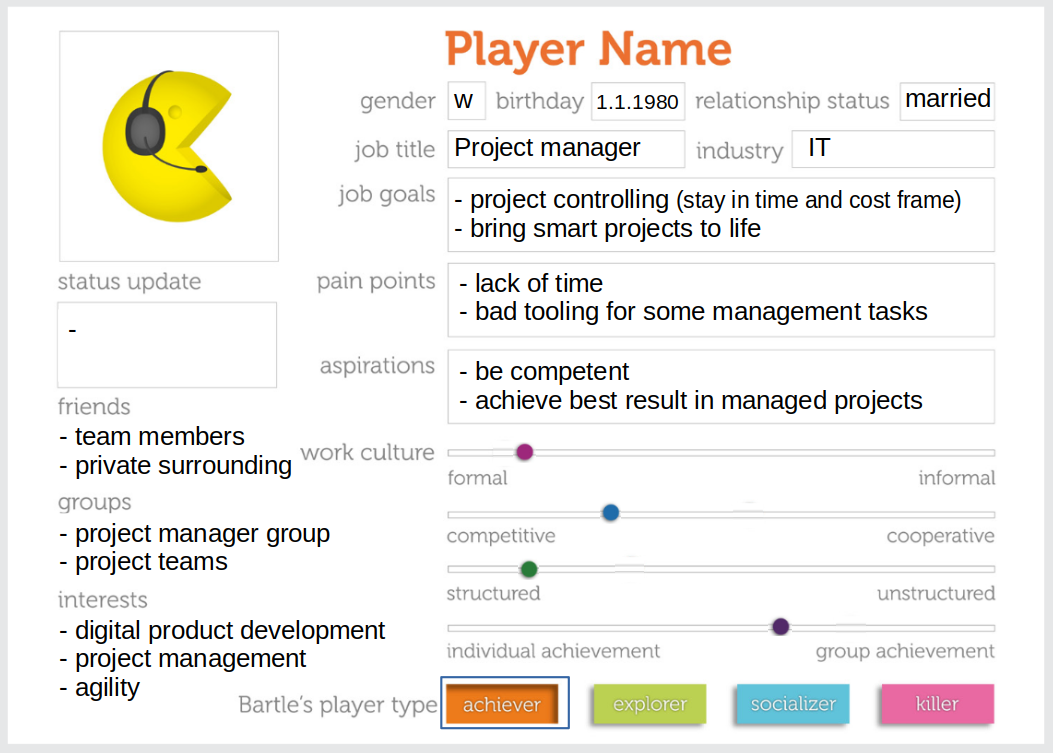
\includegraphics[width=1.0\textwidth]{Content/Domain/PersonaProjectManager.png}
	\caption{Player Persona: Project Manager}
	\label{fig:personaProjectManager}
	\cite[p. 88; adapted]{kumarGamificationWorkDesigning2013}
\end{figure}

\newpage

\paragraph*{Project Member}

The following image \ref{fig:personaProjectMember} shows the key characteristics of the project member persona.
Based on their position within the team, team members tend to be rather cooperative then competitive. Their working culture is informal and the team is oriented in reaching goals together. As a developer he is not that much interested in project management and the successful project finish in time. His main attention is drawn by a personal gain of new knowledge and an involvement in interesting projects. If the projects finish in cost and time this is rather a spin-off and not the main goal. Nevertheless in terms of project risk management he is the expert for all technical risks of the project.

\begin{figure}[H]
	\centering
	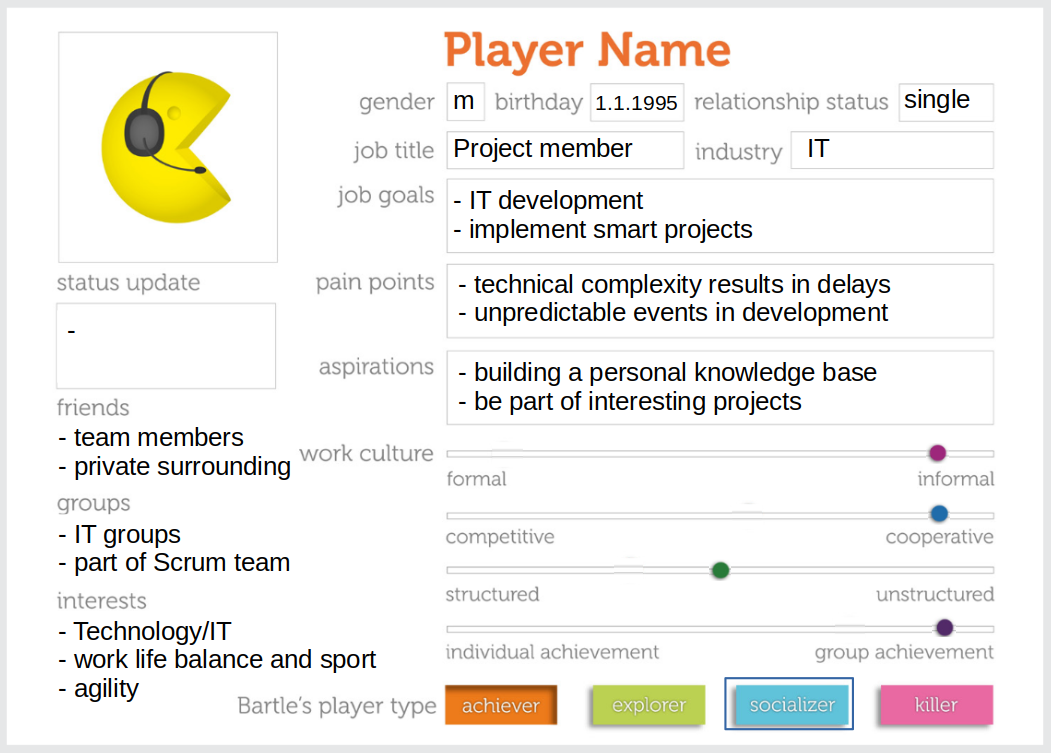
\includegraphics[width=1.0\textwidth]{Content/Domain/PersonaProjectMember.png}
	\caption{Player Persona: Project Member}
	\label{fig:personaProjectMember}
	\cite[p. 88; adapted]{kumarGamificationWorkDesigning2013}
\end{figure}


\subsection{Mission}
\label{sec:domainCb}

By defining the mission we aim to have a specific vision in mind, from which the following steps can be derived. As described in the theory chapter \ref{sec:theoryBd} the mission is defined. 
As first step the current situation was already considered  in chapter \ref{sec:theoryA}. The next step deals with the business outcome. As target business outcome we would like to lower the number of projects failing because of risk management not considered. This should be achieved by the development of a gamified application for project risk management.
Our mission is to increase the user engagement and support habit building in terms of project risk management. Especially we want to support the project managers as good as possible in their mandatory part of risk response management and monitoring (chapter \ref{sec:DomainA}).

\subsection{Mechanics}
\label{sec:domainCc}

This chapter describes the conception which mechanics from the chapter \ref{sec:theoryBc} motivational design patterns are applied.
The following mechanics have been selected for the risk management domain by us and are described in detail:
\begin{itemize}
	\item Activity Stream and Notifications
	\item Growth, Specialization—Badge and Increased Responsibility
	\item Self defined challenges
	\item Praise and Rewards (Score)
	\item Collaborative form of leaderboards
	\item Journey
	\item Social Feedback/Feedback loops
	\item Task Queue
	\item Additional minor patterns
\end{itemize}

\paragraph*{Activity Stream and Notifications}
The activity stream represents the start page and is a key component of the application. By this the user is notified about relevant changes. Furthermore the messages sent can motivate the user to directly jump into a specific workflow or task. 
It is part of the application wide engagement loop and especially accountable for the initial motivating emotion and the call to action.
%TODO ??? With notifications appearing 
%Push notifications
%-> abgewandelte form von operant conditioning mit variable ratio

The patterns used are the activity stream as social pattern and notifications as interface pattern.
The activity stream is implemented as part of \ac{UC}10 Activity Stream (\ref{sec:domainBbk}).

\paragraph*{Growth, Specialization—Badge and Increased Responsibility}

Depending on their level of interacting with the application users can be classified on the range between beginner and advanced. This can be mapped by the following five specialization—badges created by us:

project manager > risk buster > risk sage > risk master > risk owner > project member

\begin{enumerate}
	\item Project member: basic project member without any specific rights
	\item Risk owner: reached by owning a specific number of risks (being the person in charge).
	\item Risk master: reached by being part of a specific number of risk ranking processes.
	\item Risk sage: reached by reviewing and contributing a specific number of risks.
	\item Risk buster: reached by successfully contributing a specific number of risk responses.
	\item Project manager: highest achievable badge with right for creating new projects and managing existing projects.
\end{enumerate}

Growth is achieved in two areas. On the one hand specialization—badges and on the other hand the further development of project risks.

Increased responsibility is used for the process of creating and managing a project. There are two workflows how a project can be initialized. The first possibility is that a user who has reached the project manager specialization—badge creates the project. The second possibility is that at least two members insure, that one person can be a project manager.

All three patterns (Growth, Specialization—Badge, Increased Responsibility) belong to the group of gameful patterns.
They are implemented as part of \ac{UC}1 User CRUD (\ref{sec:domainBbb}), \ac{UC}2 Team Access CRUD (\ref{sec:domainBbc}), \ac{UC}6 Risk Discussion (\ref{sec:domainBbg}), \ac{UC}8 Risk Response Management (\ref{sec:domainBbi}), \ac{UC}11 Progress Indicator (\ref{sec:domainBbl}).

\paragraph*{Self defined challenges}

%TODO einbauen? -> falls ja noch Quelle suchen
%"If it doesn't challenge you it doesn't change you" - Fred Devito
Applied challenges have a positive impact while doing and after completing. While doing the user is motivated to complete the challenge. By completing challenges the users are feeling competent and their self-efficacy is increasing. A possible risk could be challenges that are too difficult and therefore demotivating. That is why we use the concept of self defined challenges. By setting the challenges by their own the probability of success is increased.

\noindent
Self defined challenges appear at several locations in the risk management application:
\begin{itemize}
	\item Project initialization (e.g. project manager defines how many risks should be contributed in a self defined time period)
	\item Risk Monitoring (e.g. daily, weekly or monthly question if preventive action was done with reminder as notification before. This tries to support habit building).
\end{itemize}

The challenges mechanic is part of the gameful patterns. 
Self defined challenges are implemented as part of \ac{UC}7 Risk Monitoring (\ref{sec:domainBbh}) and \ac{UC}9 Project initialization (\ref{sec:domainBbj}).

\paragraph*{Praise and Rewards (Score)}

Users are rewarded by points for performing desired behavior. This adds extrinsic motivational factors to the application. These mechanics are needed as a basis for a collaborative form of leaderboards (next paragraph). The collaborative leaderboard provides the user direct feedback why it is worthwhile to collect points. So praise and rewards in combination with collaborative leaderboards are trying to achieve a positive conditioning.

Points can be achieved by performing desired behavior. Desired are:
\begin{itemize}
	\item proposing risks
	\item reviewing risks
	\item be person in charge
	\item be active part of the community (e.g. contribute and manage pool risks and pool risk responses)
\end{itemize}

Praise is an interface pattern and score a gameful pattern.
Praise and rewards are implemented as part of \ac{UC}5 Risk Pool (\ref{sec:domainBbf}), \ac{UC}6 Risk Discussion (\ref{sec:domainBbg}), \ac{UC}7 Risk Monitoring (\ref{sec:domainBbh}) and \ac{UC}8 Risk Response Management (\ref{sec:domainBbi}).

\paragraph*{Collaborative form of leaderboards}

As described above the users are rewarded for desired behavior. Hence the slope of the graph (points over time) are a user activity indicator. Furthermore her/his own activity graph is easily visible for the user through the user profile page.
Instead of comparing one individual against another individual based on the points score (classical form of leaderboards) we propose a team based comparison concept. 
In detail following features are planned:
\begin{itemize}
	\item For each project team the \textbf{medium of the activity score of all project members} is calculated. This results in an activity score for each project and enables the comparison of different projects. This is done through an anonymized leaderboard (e.g. "Your project activity is currently at position X of Y projects"). Furthermore it is connected with concrete recommendations, how the position can be topped.
	%TODO: clarify if  geometrical or arithmetical mean or median
	\item The project can be classified based on the \textbf{sum of all points from each project member}. Based on this the project can be classified as "bronze", "silver" and "gold" project.
	%TODO: Concept how big teams and small teams are comparable with this approach
\end{itemize}

The important question cooperation vs. competition is already part of scientific research. Vegt et al. \cite{vegtDesigningGamificationGuide2015} have discovered, that based on the way how gamification mechanics are applied rather cooperative or competitive behavior is supported. Furthermore the team collaboration can be enhanced.

By comparing whole projects and their teams the competitive character of leaderboards is moderated and completed with cooperative elements. This strengthens the group spirit. The operativeness can be observed in team sports. The fact of being a member of a team and being able to achieve something together develops new motivation.

Leaderboards are a gameful pattern. 
The collaborative leaderboard is implemented as part of \ac{UC}2 Team Access CRUD (\ref{sec:domainBbc}) and \ac{UC}9 Project initialization (\ref{sec:domainBbj}).

\paragraph*{Journey}

By individually supporting the user while using the application one can lower the probability of disappointed users. Based on the current phase of the user (beginner, medium, advanced) the application provides different assistance. The following list depicts the specific intended actions in detail:

\noindent
Beginner level:
\begin{itemize}
	\item Introduction to the application and its aims at the first application start.
	\item Explanation of the risk discussion process.
	\item Presentation of the risk pool concept.
\end{itemize}

\noindent
Medium level:
\begin{itemize}
	\item Show path to mastery through specialization—badges and task queues.
	\item Visible feedback of the current progress through progress bars.
\end{itemize}

\noindent
Advanced level:
\begin{itemize}
	\item No disturbing information boxes about basic tasks.
	\item Increased responsibility as a project manager, clearly visible as specialization-badge for the user.
\end{itemize}

\noindent
The user journey is implemented as part of \ac{UC}11 Progress Indicator (\ref{sec:domainBbl}).

\paragraph*{Social Feedback/Feedback loops}

The core engagement loop is built onto the theory behind human motivation, behavioral psychology and behavioral economics. It tries to build a positive and motivating user experience centering the user/player. This is done by the four steps introduced in the theory chapter \ref{fig:engagementLoop}: Motivate Emotion -> Call to Action -> Re-Engage -> Feedback Reward. 

By building use cases implementing these four steps the user's motivation for doing specific tasks can be increased. Some parts of the application using the core engagement loop are listed in the following:

\begin{itemize}
	\item Risk discussion process (chapter \ref{sec:domainBbg}): Risks traverse a review and discussion process before they are added as final risks. This process is built onto social feedback and interaction between the project members.
	\item Risk adjustment process (chapter \ref{sec:domainBbe}): After adding risks they are classified by the team based on their threat probability.
	\item Progress indicators (chapter \ref{sec:domainBbl}): The application clearly makes the current state and progress visible to the user. Based on specialization-badges it is clearly visible if a user is a beginner, medium or advanced. Based on this state different support is guided by the application. E.g. if you are new to the application the risk discussion process is in need of explanation, whereas for an advanced user the process is completely clear.
	\item Risk pool (chapter \ref{sec:domainBbf}): The voting process for risks and risks responses to push it into the global risk pool makes use of the core engagement loop combined with social feedback.
\end{itemize}

Social feedback and feedback loops are implemented as part of \ac{UC}4 Risk Adjustment (\ref{sec:domainBbe}), \ac{UC}5 Risk Pool (\ref{sec:domainBbf}), \ac{UC}6 Risk Discussion (\ref{sec:domainBbg}), \ac{UC}7 Risk Monitoring (\ref{sec:domainBbh}), \ac{UC}8 Risk Response Management (\ref{sec:domainBbi}), \ac{UC}9 Project initialization (\ref{sec:domainBbj}), \ac{UC}10 Activity Stream (\ref{sec:domainBbk}) and \ac{UC}11 Progress Indicator (\ref{sec:domainBbl}).

\paragraph*{Task Queue}

Task Queues provide tasks which can be done next. In best case this supports the flow experience (described in theory chapter \ref{flow}).
They are implemented in the following parts of the application:
\begin{itemize}
	\item After proposing a risk: propose another risk, review a risk
	\item After adding a risk to the risk pool: add another pool risk, add risk response
	\item The whole process of initializing a project is guided and uses task queues
	\item After monitoring one risk: monitor another risk (if you are the person in charge)
	\item After setting a challenge: propose a challenge to a colleague
\end{itemize}

Task Queues are an Information Pattern and implemented as part of \ac{UC}5 Risk Pool (\ref{sec:domainBbf}), \ac{UC}6 Risk Discussion (\ref{sec:domainBbg}), \ac{UC}7 Risk Monitoring (\ref{sec:domainBbh}), \ac{UC}8 Risk Response Management (\ref{sec:domainBbi}), \ac{UC}9 Project initialization (\ref{sec:domainBbj}), \ac{UC}10 Activity Stream (\ref{sec:domainBbk}) and \ac{UC}11 Progress Indicator (\ref{sec:domainBbl}).

\paragraph*{Additional minor patterns}

\begin{itemize}
	\item Broadcast (e.g. Risks are shared between users)
	\item Predictable Results
	\item State Preservation
	\item Organization of Information
	\item Personalization (e.g. Risk Pool with Recommendation engine)
	\item Reporting (e.g. risks can be reported)
	\item Search (e.g. Risk Pool is searchable)
\end{itemize}


\subsection{Evaluation}
\label{sec:domainCd}

\spacing{1.5}

For evaluating the effectiveness of the gamified application for project risk management we have chosen a qualitative approach. After finishing the conception a clickable prototype was created. Based on this prototype we have evaluated the effect on real potential users through user interviews. The gained feedback and a detailed description and analysis of the user interviews can be found in chapter \ref{sec:DomainAb}.
The whole feedback was considered in the later development of the application.